\section{Unterschiedliche Ansätze der Applikationsentwicklung für mobile Engeräte}
\label{cha:3_2}
Für die Programmierung von Multi-Plattform-Applikationen gibt es unterschiedliche Ansätze, in die die Entwicklungsmethoden eingeordnet werden können. Dabei unterscheiden verschiedene Autoren unterschiedliche Ansätze. In dieser Arbeit wird dafür die von Delia et al \cite{IEEE_development_classes} definierten Einteilung verwendet. Im Folgenden werden diese vorgestellt sowie einzelne Aspekte betrachtet.

\subsection{Native Applikationen}
Native Applikationen werden entwickelt, um auf einer einzelnen Plattform eingesetzt zu werden. Der Quellcode wird dafür in ausführbaren Code übersetzt. Dieser ist spezifisch für die gewählte Plattform \cite{IEEE_development_classes}.
Die Programmierung wird in derplattformtypischen Programmiersprache geschrieben und ist dadurch nur für eine Plattform nutzbar. Es gibt folglich für jede Plattform einen eigenen Quellcode. Um etwa eine native Android App zu entwickeln, wird diese in Kotlin programmiert und im Anschluss in Kotlin-Bytecode übersetzt. Dieser Bytecode ist dabei lediglich auf Android Geräten ausführbar.

Ein Vorteil der nativen Entwicklung ist, dass die Funktionen der verschiedenen Plattform optimal genutzt werden können. Die eindeutig definierten Schnittstellen müssen dabei lediglich aufgerufen werden. So können beispielsweise Kamera, GPS oder auch Kalender einfach und effizient genutzt werden. Dabei ist die Ausführung nicht nur performant, sondern kann auch in einem Hintergrundprozess gestartet werden \cite{IEEE_development_classes}.
Zusätzlich stellen die Plattformen UI-Elemente für die native Entwicklung zur Verfügung, so dass das Aussehen der Applikation und der Benutzerschnittstellen ähnlich zu der unterstützten Plattform ist. So entsteht für den Nutzer ein geschlossenes System, das leichter zu bedienen ist, da es kaum Unterschiede in Struktur, Design, Aufbau oder auch Benutzung gibt \cite{IEEE_Khackouch_Al}.

Ein Nachteil der nativen Entwicklung von Multi-Plattform Anwendungen ist der Aufwand und die damit verbundenen Kosten. Da die Anwendung für jede Plattform einzeln verwirklicht werden muss. So können die Gesamtkosten durch die Multiplikation der Entwicklungskosten einer Plattform mit der Anzahl der zu unterstütztenden Plattformen geschätzt werden \cite{IEEE_Khackouch_Al}. Doch nicht nur die initiale Implementierung ist kostenintensiv. So nennen Delia et al \cite{IEEE_development_classes} auch das Testen, Abändern und Verteilen neuer Versionen als Kosten, die auf jeder unterstützten Plattform auftreten. 
Um die Kosten zu verringern, können deswegen anfänglich einzelne Plattformen zur Implementierung ausgewählt werden, wodurch jedoch die Zahl der potentiellen Nutzer sinkt.

\subsection{Web-Applikationen}
\label{cha:3_2_web}
Web-Applikationen sind Applikationen, die im Internet verfügbar sind. Sie sind darauf ausgelegt, als Webanwendungen auf einem Server zu laufen und dann mittels eines Browser auf dem Geräte aufgerufen zu werden. Der Nutzer kann ohne zusätzliche Installation die Anwendung nutzen, sobald der Server gestartet wurde \cite{IEEE_Khackouch_Al}.
Da sie auf allen Geräten mit einem Browser und einer Internetverbindung aufgerufen werden kann, müssen keine plattformspezisfischen Versionen entwickelt werden.
So können alle Plattformen mit nur einer Entwicklung abgedeckt werden \cite{IEEE_development_classes}.

Wie bereits erwähnt, können Entwicklungskosten gesparrt werden, da nur ein Code für alle Plattformen geschrieben wird. Ein weiterer Vorteil ist, dass Updates dem Nutzer direkt nach einem Neustart des Servers zur Verfügung stehen, da diese nicht erst an die Geräte verteilt und dann installiert werden müssen \cite{IEEE_Khackouch_Al}. Des Weiteren können mittlerweile selbst Laien Webseiten erstellen, da Firmen wie beispielsweise Squarespace\footnote{https://de.squarespace.com/} die Erstellung stark vereinfacht. So muss gerade einmal eine Vorlage ausgewählt werden und das Design auf das Projekt angepasst werden, um eine nutzbare Webanwendung zu erhalten. 
Außerdem kann der Code einer Webapplikation wiederverwendet werden, um etwa eine hybride Applikation, wie sie ihn Kapitel \ref{cha:3_hybrid} erklärt wird, zu erstellen \cite{IEEE_Khackouch_Al}. 

Jedoch ist die nutzbare Funktionalität der Plattform, durch die Beschränkungen des genutzten Browsers limitiert. Dabei können lediglich die Funktionalitäten genutzt werden, auf welche der Browser Zugriff hat \cite{Phyo}. Hinzukommend tritt bei einer langsamen Internetverbindung eine erhöhte Ladezeit auf und infolge dessen sinkt die Performance. Wenn eine Internetverbindung gänzlich nicht verfügbar ist, so kann die Anwendung gar nicht genutzt werde \cite{IEEE_Khackouch_Al}. Des Weiteren müssen Webanwendungen zur Nutzung auf Smartphones angepasst werden, um auf unterschiedliche Seitenverhältnisse und Auflösungen reagieren zu können. So sind Smartphones etwa höher als breit und haben daher weniger Platz in der Menüleiste als etwa bei einer Nutzung an einem Computer. Folglich muss abhängig der Bildschirmauflösung ein angepasstes Design zur Verfügung gestellt werden \cite{Serrano_mobile}.

Web-Applikationen sind in den letzten Jahren, durch die Verfügbarkeit von schnellen Internetverbindungen in fast allen Teilen der Welt, einfacher nutzbar geworden.
Im Schnitt stieg die mobile Bandbreite zwischen 2017 und 2021 um 59,5\% beziehungsweise von knapp 20 Mbps auf 55 Mbps\footnote{https://www.ookla.com/articles/global-index-2019-internet-report}.
Jedoch ergab eine Studie von Yoram Wurmser \cite{report_webusage}, dass während der Nutzung des Smartphones, amerikanische Erwachsene etwa 89\% der Zeit in Applikationen und gerade einmal 11\% in einem Browser verbringen.

\subsection{Hybride Applikationen}
\label{cha:3_hybrid}
Der Ansatz der Entwicklung einer hybriden Applikation teil viele Eigenschaften mit den Web-Applikationen.
Sie nutzen Web-Technologien wie beispielsweise HTML, Javascript und CSS, werden jedoch in einer Applikation mit einem Webcontainer nicht im Browser des Geräts ausgeführt \cite{IEEE_development_classes}.
Sie verfügt hierbei über eine Schnittstelle mittels welcher sie Zugriff auf die Funktionalität der Plattform erhält.

\begin{figure}[ht]
  \centering
  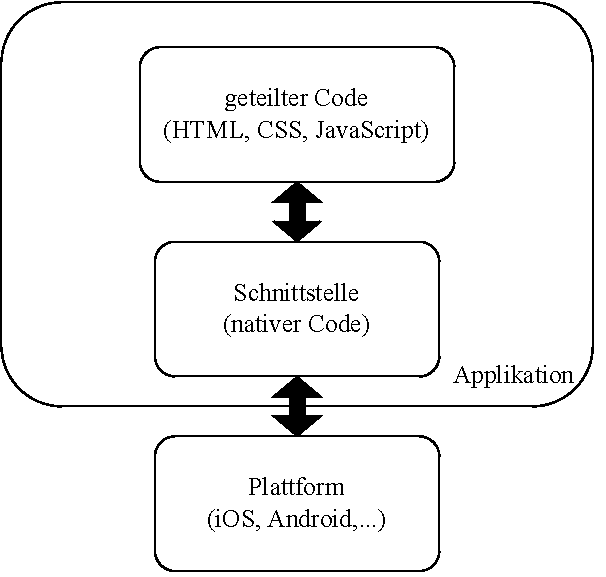
\includegraphics[height=8cm,keepaspectratio]{images/hybrid_architecture.drawio.pdf} 
  \caption{Architektur einer hybriden Applikationen}
  \label{fig:hybrid_architecture}
\end{figure}

Wie in Abbildung \ref{fig:hybrid_architecture} zu sehen ist, besteht diese Art von Applikation aus zwei Teilen.
Der erste Teil ist ein geteilter Code, der mit Web-Technologien erstellt wird und sowohl die UI als auch Applikationslogik enthält. Der geteilte Code kann dabei sowohl lokal als auch auf einem Server gespeichert werden und ist für mehrere Plattformen verwendbar \cite{2017hybrid_approach_end}.
Der zweite Teil formt eine Schnittstelle, die in nativen plattformspezifischen Code geschrieben ist. Der Schnittstellencode kann etweder selbstständig implementiert werden oder von einem Schitstellen Framework wie Cordova\footnote{https://cordova.apache.org/} zur Verfügung gestellt werden. Die Schnittstelle verwirklicht eine bidirektionale Kommunikation zwischen der Plattform und der Applikationslogik \cite{ELKASSAS2017163}. Somit kann die Anwendung auf die Funktionalitäten der Plattform zugreifen. Zusätzlich ermöglicht sie die Darstellung der Anwendung auf dem Endgerät. 

Grundsätzlich teilt dieser Ansatz die gleichen Vor- und Nachteile wie Web-Applikationen, da sie zu einem großen Teil die selbe Technologie nutzt. Jedoch kann eine offline Funktionalität erreicht werden, wenn die Anwendung lokal gespeichert ist. Zusätzlich erhält die Applikation durch die Schnittstelle Zugriff auf die native Funktionalität und kann auf dem Gerät installiert werden. Weiterhin kann der geteilte Code sowohl auf den verschiedenen Plattformen, als auch in anderen Technologien wiederverwendet werden, da es sich im Prinzip um eine Webseite innerhalb einer Applikation handelt \cite{IEEE_development_classes}. Jedoch entsteht durch den zusätzlichen Web-Container, der geladen werden muss um die UI anzuzeigen, eine erhöhte Ladezeit, die sich negativ auf die Performance der Applikation auswirkt \cite{IEEE_development_classes}.

\subsection{Interpretierte Applikationen}
\label{cha:3_2_interpretiert}
Bei interpretieren Cross-Plattform Anwendungen schreibt der Entwickler Code, der anschließend mithilfe eines Interpreters während der Laufzeit in ausführbaren Code übersetzt wird. Folglich besteht die auf dem Gerät installierte Anwendung aus zwei Teilen. Zum einen einem nativen Teil, oftmals Frameworkcode, der zum Übersetzen der eigentlichen Anwendung benötigt wird. Zum anderen einen Cross-Plattform Teil, der die Anwendungslogik realisiert \cite{IEEE_development_classes}.

Der Unterschied zu einer hybriden Applikation besteht darin, dass die Anwendungen je nach Plattform anders aussehen können. So wird etwa die Benutzeroberfläche nicht so angezeigt, wie sie im Code definiert ist, sondern wird erst während der Laufzeit in eine native UI übersetzt.
Dadurch wird eine Nutzung von nativen Elementen möglich, obwohl die Anwendung eigentlich in einer anderen Sprache definiert ist \cite{IEEE_development_classes}. 
Dazu kommt, dass eine Anwendungen auf allen Plattformen ausgeführt werden kann, die von dem entsprechenden Interpreter unterstützt wird \cite{server_side}.

Dadurch ergibt sich jedoch eine Abhängigkeit zum Framework und dessen unterstützten Plattformen. Zudem hat durch die Interpretierung während der Laufzeit dieser Ansatz eine hohe Reaktionszeit, da jede Zeile vor Ausführung erst durch den Interpreter übersetzt werden muss und somit eine extra Latenz zwischen jedem einzelnen Aufruf und dessen Ausführung entsteht \cite{server_side}.

\subsection{Cross-kompilierte Applikationen}
Bei cross-kompilierten Applikationen wird während der Entwicklung ebenfalls lediglich ein Quellcode geschrieben, jedoch wird dieser bereits vor Verteilung in nativen Code übersetzt. Daher muss der Übersetzungsprozess nur einmalig durchgeführt werden und nicht wie bei dem interpretierten Ansatz bei jeder Benutzung. Um dies zu erreichen, wird ein Cross-Compiler benötigt, der für mehrere unterschiedliche Plattformen Kompilate erzeugt \cite{mobiledraft_cross_plattform}. Somit kann aus einem Code für jede Plattform eine eigene Anwendung gebaut werden, die ausschließlich aus nativem Code besteht und sich folglich für das Betriebssystem nicht von einer nativen Anwendung unterscheidet \cite{IEEE_development_classes}.Im Vergleich zur interpretieren Anwendung kann außerdem die App-Größe reduziert werden, da kein zusätzlicher Übersetzer benötigt wird \cite{mobiledraft_cross_plattform}.

Auch bei diesem Ansatz ist die Funktionalität und die Zahl der unterstützten Plattformen von dem genutzten Cross-Compiler abhängig. Einige dieser Frameworks nutzen eine spezialisierte Programmiersprache, sodass eine Wiederverwendung des Codes, für einen anderen Ansatz, erschwert wird. So wird bei Flutter\footnote{https://flutter.dev/} die Sprache Dart\footnote{https://dart.dev/} und bei Xamarin\footnote{https://dotnet.microsoft.com/en-us/apps/xamarin} Lua\footnote{https://www.lua.org/} genutzt.


\subsection{Gemischter Ansatz}
In dieser Arbeit sollen die Applikationsklassen um einen weiteren Ansatz erweitert werden, wie ihn Khachouch et al \cite{IEEE_Khackouch_Al} in ihrere Arbeit aufführen. Sie definieren einen gemischten Ansatz, um die verschiedenen Ansätze kombiniert zu können, Somit können die Vorteile unterschiedlicher Ansätze vereint werden,
